\subsubsection{Taxi Driver Reporting}
			To accompany this diagram, read the Scenario \hyperref[sec:TaxiDriverReportingScenario]{S.7}.

				\begin{table}[htpb]
					\centering
					\label{tab:TaxiDriverReportingDiagramTable}
					\begin{tabularx}{\textwidth}{lp{9cm}}
						\hline
						\hline
							\textbf{Subject}
						& 
							\textbf{Description}\\
						\hline
							Actors	       &  Customer, myTaxiService Mobile Application, myTaxiService Server\\
						\hline
							Preconditions  &  Customer must be logged in.\\
						\hline
							Execution      &  1.~Customer open the myTaxiService Mobile Application.\\
										   &  2.~Customer taps on the "Request Taxi" button.\\
										   &  3.~myTaxiService Mobile Application send the requests to the Server.\\
										   &  4.~Customer waits for the acceptance.\\
										   &  5.~myTaxiService Mobile Application shows the acceptance notification.\\
										   &  6.~Customer waits for the Taxi that does not arrive.\\
										   &  7.~Customer ends the ride reporting the Taxi Driver.\\
						\hline
							Postconditions &  The ride is set to ended and the Taxi Driver is reported.\\
						\hline
							Exceptions     &  1.~The Custoemr disconnects before reporting.\\
									
						\hline
						\hline
					\end{tabularx}
				\end{table}
				
				\begin{figure}[H]
					\centering
					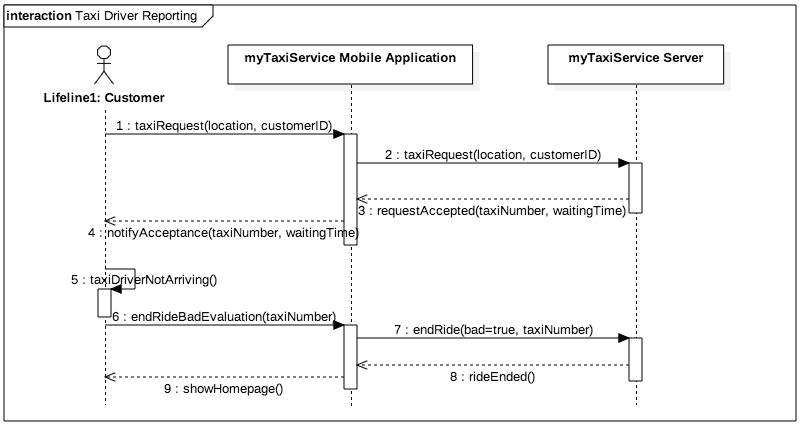
\includegraphics[width=\textwidth, scale=0.5]{IMG/InteractionDiagrams/TaxiDriverReporting.png}
					\caption{Taxi Driver Reporting Interaction Diagram}\label{sec:FigureTaxiDriverReporting}
				\end{figure}